\documentclass{article}
\usepackage{graphicx} % Required for inserting images

\title{DCT-REM}
\author{Yongjian Zhao}
\date{March 2026}
\usepackage{algorithmic}
\usepackage{algorithm}
\usepackage{array}
\usepackage[caption=false,font=normalsize,labelfont=sf,textfont=sf]{subfig}
\usepackage{amsmath,amssymb,amsfonts}


% ---------- Layout and Graphics ----------

\usepackage{graphicx}
\usepackage{adjustbox}
\usepackage{textcomp}
\usepackage{siunitx}
\usepackage{textcomp}
\usepackage{stfloats}
\usepackage{url}
\usepackage{verbatim}

\usepackage{array,booktabs,tabularx}
\usepackage{multirow}
\usepackage{hyperref}
\usepackage{adjustbox}
\newcommand{\cmark}{\ding{51}}  % ✓
\newcommand{\xmark}{\ding{55}}  % ✗
\usepackage{pifont}                  % \ding symbols
\newcommand{\fstar}{\ding{72}}       % filled star
\newcommand{\hstar}{\ding{73}}       % hollow star
\newcolumntype{C}[1]{>{\centering\arraybackslash}p{#1}}
\renewcommand{\arraystretch}{1.15}

% ---------- Colors and Citations ----------
\usepackage{xcolor}                              % ← Must load first
\definecolor{labelblue}{RGB}{0,0,180}
\definecolor{numberblue}{RGB}{0,0,180}

\makeatletter                                     % ← Disable natbib hook
\let\NAT@parse\undefined
\makeatother

\usepackage[capitalize]{cleveref}                % ← Load cleveref after hyperref
\usepackage[numbers]{natbib}

% ===== cleveref unified styling =====
% equation
\crefname   {equation}{\textcolor{labelblue}{Equation.}}{\textcolor{labelblue}{Equations.}}
\Crefname   {equation}{\textcolor{labelblue}{Equation.}}{\textcolor{labelblue}{Equations.}}
\creflabelformat{equation}{\textcolor{numberblue}{(#2#1#3)}}

% figure
\crefname   {figure}  {\textcolor{labelblue}{Fig.}}     {\textcolor{labelblue}{Figs.}}
\Crefname   {figure}  {\textcolor{labelblue}{Fig.}}     {\textcolor{labelblue}{Figs.}}
\creflabelformat{figure}{\textcolor{numberblue}{#2#1#3}}

% table
\crefname   {table}   {\textcolor{labelblue}{Table.}}   {\textcolor{labelblue}{Tables.}}
\Crefname   {table}   {\textcolor{labelblue}{Table.}}   {\textcolor{labelblue}{Tables.}}
\creflabelformat{table}{\textcolor{numberblue}{#2#1#3}}

% algorithm
\crefname   {algorithm}{\textcolor{labelblue}{Algorithm.}}{\textcolor{labelblue}{Algorithms.}}
\Crefname   {algorithm}{\textcolor{labelblue}{Algorithm.}}{\textcolor{labelblue}{Algorithms.}}
\creflabelformat{algorithm}{\textcolor{numberblue}{#2#1#3}}

% ---------- Others ----------
\hyphenation{op-tical net-works semi-conduc-tor IEEE-Xplore}

\begin{document}

\maketitle

\section{DCT-Based Servo Control Algorithm Design}
\label{sec:algorithm}

A visual servoing framework leveraging DCT is proposed to robustly extract and control visual features under specific photoacoustic (PA) imaging constraints. This section briefly outlines the integration of standard spectral transformations before detailing our primary innovation: the formulation of a frequency-domain interaction matrix tailored to PA geometry, culminating in a hybrid 6-DoF dual-sensor servoing framework utilizing an Intel RealSense camera for robust out-of-plane compensation.

\subsection{Spectral Feature Representation (Condensed Background)}
\label{sec:Spectral_Feature_Representation}

Traditional image-based visual servoing (IBVS) regulates robotic motion by minimizing the feature-space discrepancy between current sensor data and desired target configurations. However, conventional IBVS relies on spatial pixel intensities, exhibiting heightened noise sensitivity and significantly constrained convergence domains when applied to medical ultrasound and PA imaging. PA visual servoing is further exacerbated by laser-limited frame rates and non-stationary electromagnetic interference.

To overcome these modality-specific limitations, our methodology bypasses spatial intensity features, directly transforming the PA region of interest (ROI) into the frequency domain. Utilizing the well-established 2D Discrete Cosine Transform (DCT) \cite{ahmed2006discrete}, we map spatial intensities into a frequency coefficient matrix. By employing a standard zigzag scanning protocol (illustrated in \Cref{fig:feature_construction}(c)), we prioritize low-frequency components, extracting a compact visual feature vector \(\boldsymbol{s}(u,v) \in \mathbb{R}^K\). This spectral truncation acts as an inherent low-pass filter (as demonstrated in \Cref{fig:DCT_transform}), retaining macroscopic vascular topology while discarding the high-frequency interference characteristic of raw PA signals.

\begin{figure}[!htb]
    \centering
    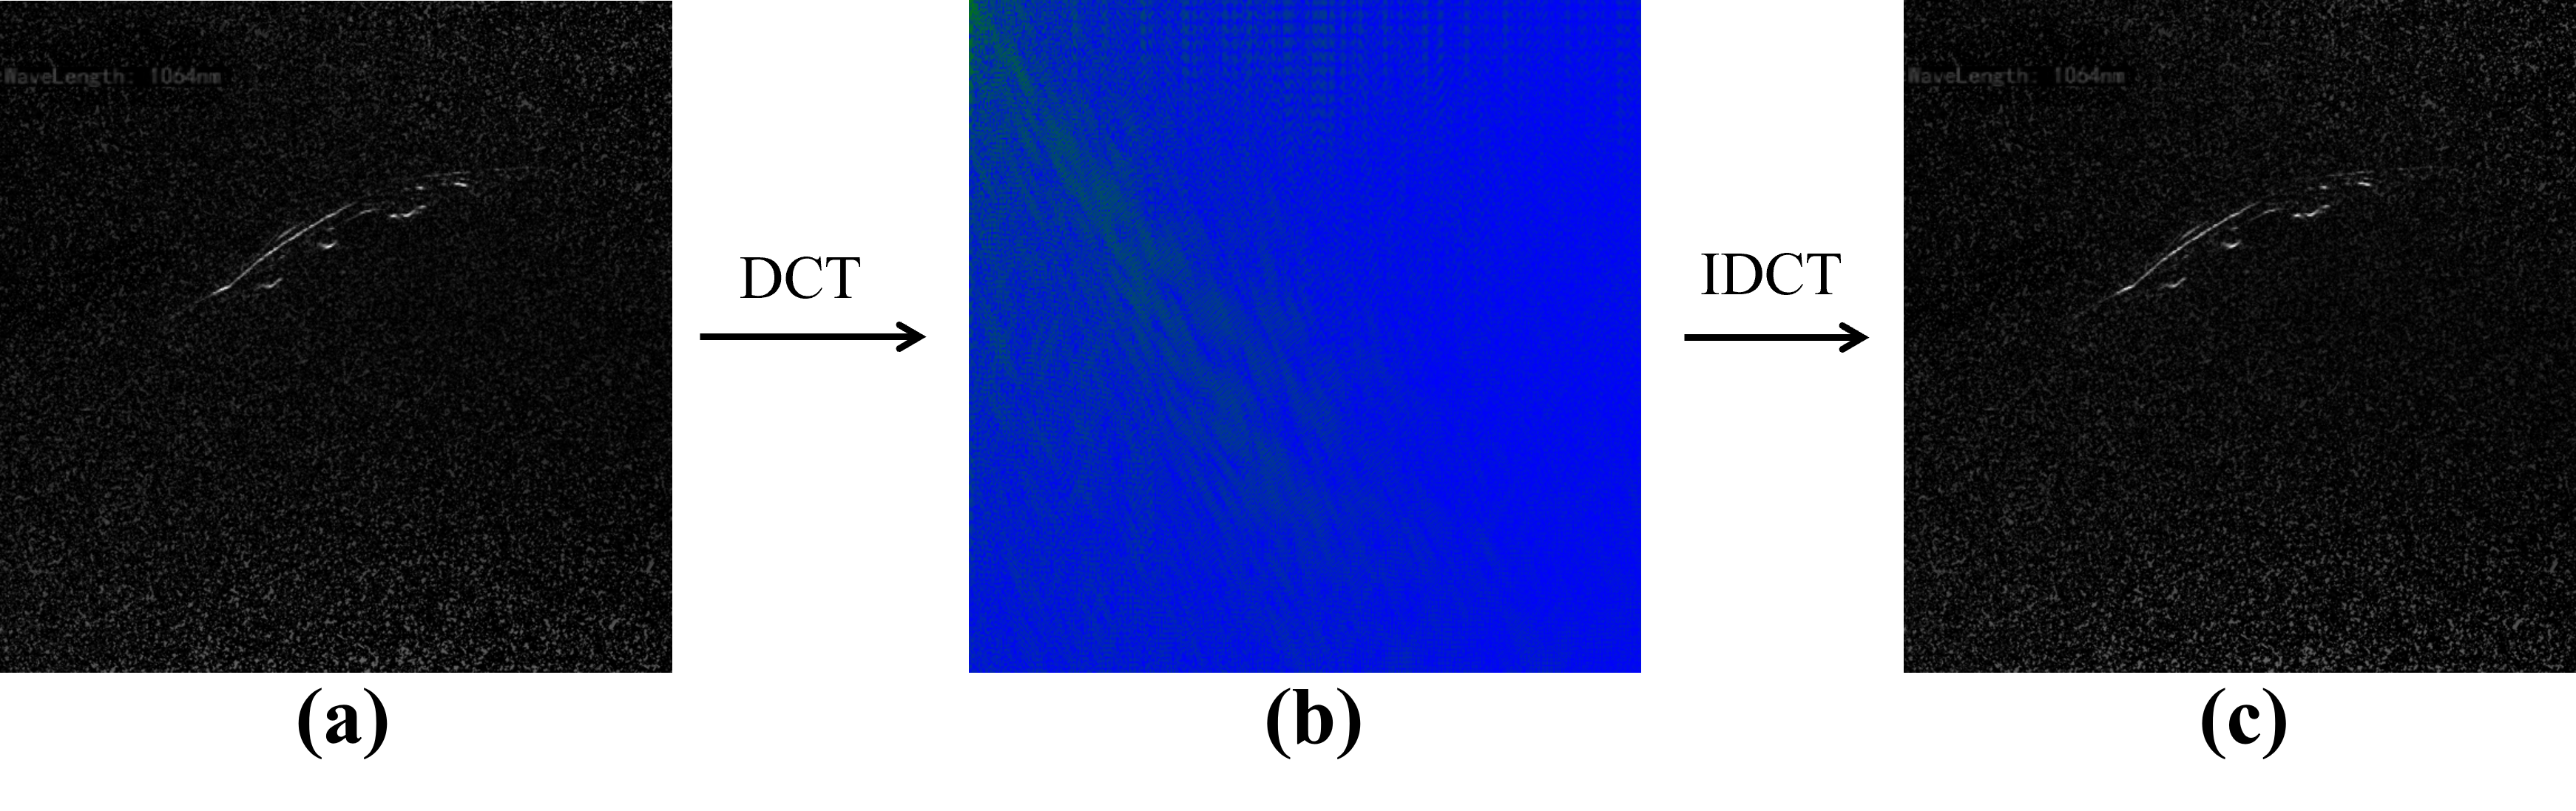
\includegraphics[width=\columnwidth]{graph/IDCT_new.png}
    \caption{Spectral decomposition and reconstruction via Discrete Cosine Transform: 
    (a) Original spatial-domain vascular image \(\boldsymbol{I}(x, y)\), 
    (b) Frequency-domain coefficient matrix \(\boldsymbol{F}(u, v)\) showing characteristic energy compaction in low-frequency quadrant, 
    (c) Perfect reconstruction through IDCT validating transformation integrity and noise preservation properties.}
    \label{fig:DCT_transform}
\end{figure}

\begin{figure*}[htbp]
    \centering
    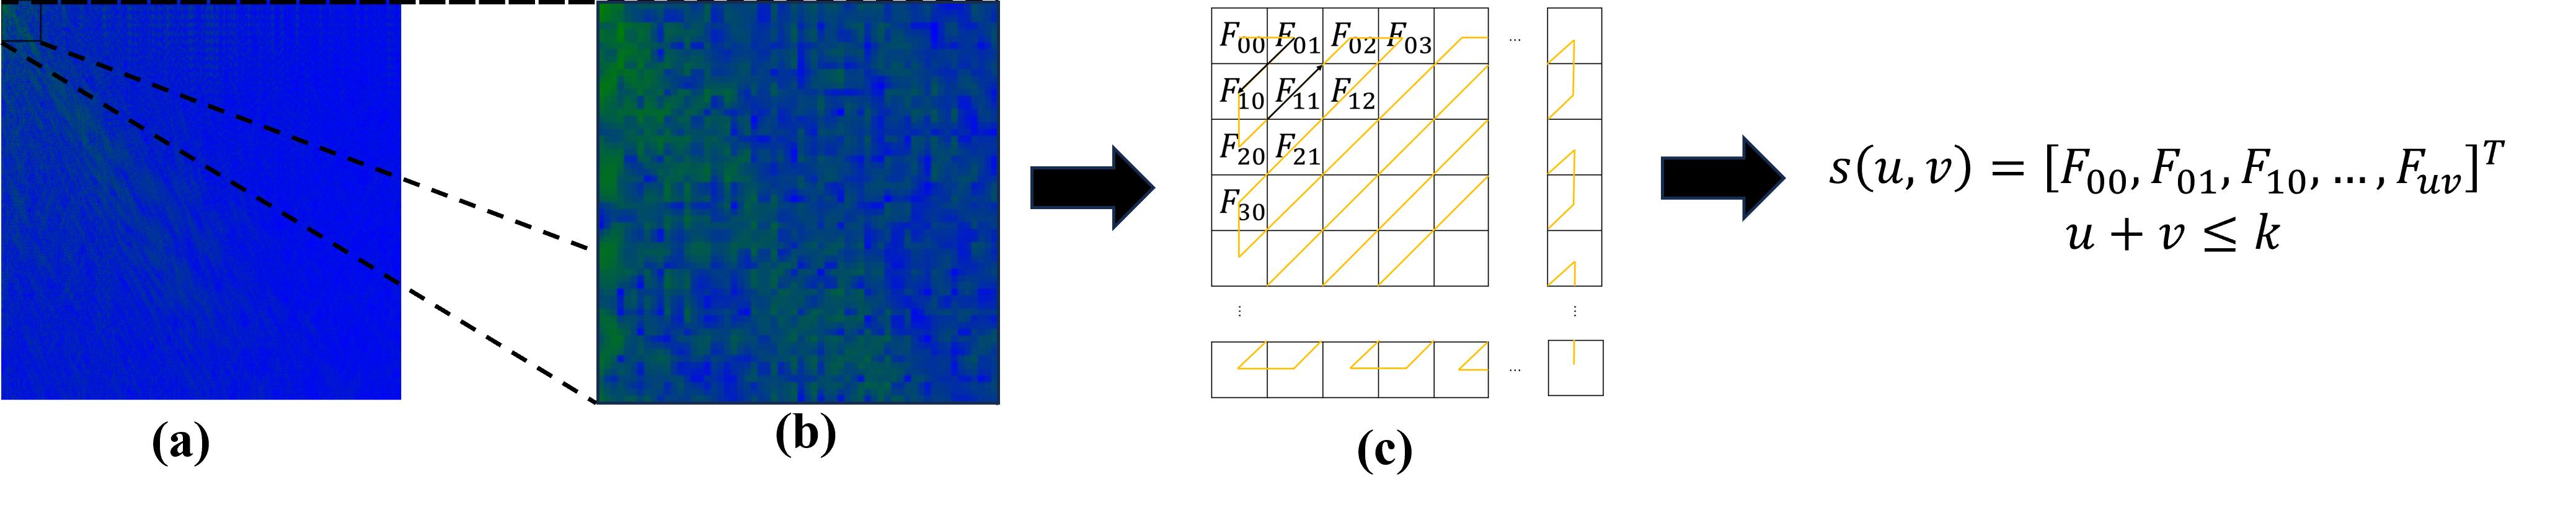
\includegraphics[width=1\textwidth]{graph/spatial calibration.png}
    \caption{Frequency-domain visual feature construction methodology: 
    (a) 2D DCT coefficient spectrum showing spectral energy concentration in low-frequency quadrant (\(u,v < 5\)), 
    (b) Magnified visualization of low-frequency region (\(0 \leq u,v \leq 15\)) demonstrating energy compaction property, 
    (c) Zigzag scanning protocol selecting coefficients satisfying \(u + v \leq k\) to construct compressed feature vector:  
    \(\boldsymbol{s}(u,v) = [F_{00}, F_{01}, F_{10}, \dots, F_{uv}]^\top \in \mathbb{R}^K\).}
    \label{fig:feature_construction}
\end{figure}

\subsection{PA-Optimized Interaction Matrix Construction}
\label{sec:PA-Optimized_Interaction_Matrix}

While traditional IBVS relies on camera data projected from 3D scenes onto 2D planes via pinhole models, PA visual servoing operates under fundamentally different image formation mechanics. PA images represent 2D cross-sectional views; structural features are only acquired when they intersect the specific PA beam plane \cite{nadeau2013intensity}.

We define the imaging plane (probe plane) as the coordinate system \(\mathcal{F}_p\) with its origin at the image center \(P(u_0, v_0)\). The \(y_p\)-axis aligns with the PA propagation direction, and the \(z_p\)-axis is normal to the image plane. Under this geometry, a physical point \(\mathbf{P_X} = (P_X, P_Y, 0)\) maps to pixel coordinates \((u, v)\) via the intrinsic scaling factors \(\alpha_u\) and \(\alpha_v\).

Under the assumptions of a stationary environment and constant photoacoustic reflection, we differentiate the frequency-domain features with respect to time to map the differentials \(\dot{\boldsymbol{s}}_{(u,v)}\) to the 6-DoF probe velocity \(\mathbf{v}_c \in \mathbb{R}^6\):
\begin{equation}
\dot{\boldsymbol{s}}_{(u,v)} = \boldsymbol{L}_{\boldsymbol{s}_{(u,v)}} \mathbf{v}_c
\end{equation}

Unlike conventional photometric interaction matrices, our formulation specifically computes the gradient mapped through the PA probe's spatial scaling geometry. The resulting interaction matrix \(\boldsymbol{L}_{\boldsymbol{s}_{(u,v)}}\) for each spectral coefficient establishes a robust linear mapping that is resilient to out-of-plane artifacts:
\begin{equation} \label{eq:L_s_uv}
	\begin{aligned}
		\boldsymbol{L}_{s_{(u,v)}} = 
		& \left[\nabla s_x \quad \nabla s_y \quad \nabla s_z \quad y\nabla s_z \right. \\
		&\left.\; -x\nabla s_z \quad x\nabla s_y - y\nabla s_x\right]
	\end{aligned}
\end{equation}

By aggregating the interaction rows for all retained zigzag indices, we construct the global interaction matrix \(\boldsymbol{L}_s \in \mathbb{R}^{K \times 6}\).

\subsection{Adaptive Control Law for Vascular Surveillance}
\label{sec:Adaptive_Control_Law}

To balance terminal precision with the computational latency induced by high-order features, we introduce an adaptive order selection strategy where the coefficient count \(K\) dynamically scales based on the exponential decay of the mean squared error between current and target features:
\begin{equation}
K = \left(K_{\max} - K_{\min}\right) \eta + K_{\min}, \quad \eta \in [0, 1], \quad K \in \mathbb{N},
\end{equation}
where the adaptation parameter \(\eta\) is defined by the initial error \(\bar{e}_s^0\) and current error \(\bar{e}_s\):
\begin{equation}
\eta = \frac{\bar{e}_s^0}{\bar{e}_s^0 + \lambda_\eta \, \bar{e}_s}.
\end{equation}

To guarantee convergence stability amidst dynamic feature counts, the in-plane robotic velocity commands are executed using a Levenberg-Marquardt inspired control formulation that adaptively weights the gradient information \cite{dame2009entropy,collewet2011photometric,marchand2019subspace}.

\subsection{Dual-Sensor Hybrid 6-DoF Servoing Framework}
\label{sec:Hybrid_Servoing}

A single 2D PA cross-section intrinsically lacks unique observability for out-of-plane motions (i.e., normal distance $v_z$, pitch $\omega_x$, and yaw $\omega_y$). To achieve robust 6-DoF robotic imaging, we integrate an Intel RealSense depth camera, establishing a two-stage "Global PBVS Guidance + Local Hybrid Dual-Servoing" strategy.

\subsubsection{Two-Stage Strategy and DoF Decoupling}
\textbf{Phase I: Global Target Guidance.} Prior to PA signal acquisition, the system relies on RGB-D data. Position-based visual servoing (PBVS) guides the PA probe directly above the target region and aligns it with the skin surface normal until the optimal working distance is reached.

\textbf{Phase II: Decoupled Dual-Servoing.} Once the PA image appears, the system transitions into a hybrid mode. The 6-DoF twist command is decoupled based on orthogonal sensor spaces (\Cref{tab:dof_mapping}):
\begin{itemize}
    \item \textbf{In-plane (DCT-PAVS):} Regulates $v_x, v_y, \omega_z$ to accurately align vascular cross-sections using DCT features.
    \item \textbf{Out-of-plane (PBVS):} Regulates $v_z, \omega_x, \omega_y$ utilizing RealSense depth data to maintain constant contact distance and normal posture, actively compensating for patient respiratory disturbances.
\end{itemize}

\begin{table}[htpb]
\centering
\caption{DoF Decoupling and Feedback Mapping in the Hybrid System}
\label{tab:dof_mapping}
\begin{tabular}{@{}C{1.5cm}C{1.5cm}C{2.5cm}l@{}}
\toprule
\textbf{DoF} & \textbf{Servo Type} & \textbf{Feedback Source} & \textbf{Control Objective} \\ \midrule
$v_x, v_y$ & IBVS & PA DCT features $s(I)$ & In-plane cross-section translation \\
$\omega_z$ & IBVS & PA DCT features $s(I)$ & In-plane cross-section rotation \\
$v_z$ & PBVS & RealSense Depth & Maintain constant standoff $d^*$ \\
$\omega_x, \omega_y$ & PBVS & RealSense Normal $\mathbf{n}$ & Out-of-plane posture alignment \\ \bottomrule
\end{tabular}
\end{table}

\subsubsection{Hybrid Control Law Formulation}
Let the synthesized 6-DoF end-effector twist be denoted as $\mathbf{u} = [v_x, v_y, v_z, \omega_x, \omega_y, \omega_z]^\top$.

For the in-plane PA control, the velocity command $\mathbf{u}_{PA} = [v_x, v_y, \omega_z]^\top$ is derived from the feature error $\mathbf{e}_{PA}$:
\begin{equation}
\mathbf{u}_{PA} = -\lambda_{PA} \mathbf{L}_{PA}^+ \mathbf{e}_{PA}
\end{equation}
where $\mathbf{L}_{PA}$ is the reduced interaction matrix containing only the columns corresponding to $v_x, v_y, \omega_z$.

For the out-of-plane PBVS, let $d$ be the measured normal distance and $\mathbf{n} = [n_x, n_y, n_z]^\top$ be the unit normal vector of the skin surface. Defining the distance error $e_z = d - d^*$ and the orientation error $\mathbf{e}_{ori} = \mathbf{n} \times [0,0,1]^\top = [n_y, -n_x, 0]^\top$, the compensation twist $\mathbf{u}_{RS} = [v_z, \omega_x, \omega_y]^\top$ is:
\begin{equation}
\mathbf{u}_{RS} = -\lambda_{RS} \begin{bmatrix} e_z \\ n_y \\ -n_x \end{bmatrix}
\end{equation}

The final 6-DoF command executed by the robot is the direct synthesis of these decoupled laws:
\begin{equation}
\mathbf{u} = \begin{bmatrix} \mathbf{u}_{PA}(1), & \mathbf{u}_{PA}(2), & \mathbf{u}_{RS}(1), & \mathbf{u}_{RS}(2), & \mathbf{u}_{RS}(3), & \mathbf{u}_{PA}(3) \end{bmatrix}^\top
\end{equation}

\subsubsection{Decoupling and System Stability Analysis}
In hybrid servoing frameworks, multi-sensor feedback often induces control interference. However, our proposed framework exhibits natural orthogonal decoupling under local contact geometry. 

The physical slicing mechanism of PA imaging restricts its sensitivity exclusively to the in-plane motion subspace $\mathcal{V}_{in} = \{v_x, v_y, \omega_z\}$. Conversely, the geometric constraints extracted by the RealSense camera strictly govern the out-of-plane motion subspace $\mathcal{V}_{out} = \{v_z, \omega_x, \omega_y\}$. Because these subspaces are disjoint in Euclidean space ($\mathcal{V}_{in} \cap \mathcal{V}_{out} = \emptyset$), the global interaction matrix $\mathbf{L}_{global}$ forms an ideal block-diagonal structure:
\begin{equation}
\mathbf{L}_{global} = 
\begin{bmatrix}
\mathbf{L}_{PA} & \mathbf{0} \\
\mathbf{0} & \mathbf{L}_{RS}
\end{bmatrix}
\end{equation}
Consequently, the error descent gradients for both tasks are orthogonal within the Lie algebra $se(3)$ space. Based on Lyapunov stability theory, simultaneously minimizing the PA feature error and the geometric spatial error guarantees local asymptotic stability without inducing coupling oscillations. This physical decoupling actively suppresses respiratory disturbances out-of-plane without jeopardizing the precise in-plane vascular alignment, fulfilling the stringent requirements of longitudinal surveillance.

\bibliographystyle{IEEEtran}
\bibliography{references}

\end{document}